\documentclass[12pt]{beamer}
\usepackage[utf8]{inputenc}
\usepackage[portuguese]{babel}
\usepackage{graphicx}
\graphicspath{{./images}}
\usepackage{colortbl}
\usepackage{color}
\usepackage{cite}
\usepackage{breqn}
%\usepackage[clean]{svg}

\definecolor{azul}{rgb}{0,0,.5}
\setbeamertemplate{navigation symbols}{}

\usetheme{Frankfurt}
\usecolortheme[named=azul]{structure}

%% Definindo o Autor e o título
\newcommand{\prof}{Claudio R. M. Mauricio}
\newcommand{\materia}{Processamento de Imagens Digitais}

\author[Aluno:~Victor E. Almeida]{Victor Emanuel Almeida}

\title{Filtros e técnicas básicas de \materia}
\subtitle{Demonstrando o software}
\date{\today}
\institute{UNIOESTE}

\begin{document}
\frame{\titlepage}

\begin{frame}
\frametitle{Conteúdo}
\tableofcontents
\end{frame}

\section{Introdução}\label{Introdução}
\begin{frame}
    \frametitle{Softwares utilizados}
    \begin{itemize}
    \item\textbf{Linguagem de programação}: C++;
    \item\textbf{Framework para interfaces gráficas}: wxWidgets\cite{docsWx};
    \item\textbf{Framework para visão computacional}: opencv\cite{docsCv};
    \end{itemize}
\end{frame}

\section{Estrutura do projeto}\label{Estrutura do projeto}
\begin{frame}
    \frametitle{Principais classes}
    % Dentro da classe app que é a classe principal
    % Tem a chamada para o main frame...
    \begin{itemize}
        \item App;
        \item MainFrame;
        \item ImagePanel;
        \item ImageHistory;
        \item Image;
    \end{itemize}
\end{frame}

\begin{frame}
    \frametitle{Representando graficamente}

    \begin{figure}
        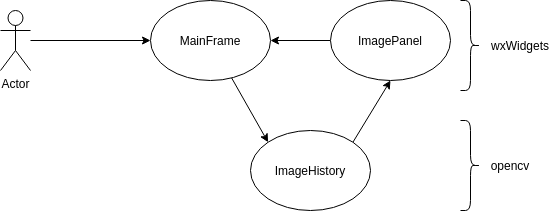
\includegraphics[width=.9\linewidth]{flow.png}
        %\includesvg[width=\linewidth]{flow.svg}
    \end{figure}

\end{frame}

\section{Métodos disponíveis}\label{Métodos disponíveis}
\begin{frame}
    \frametitle{Menus disponíveis na interface}
    \begin{itemize}
        \item Imagem;
        \item Filtros;
        \item Detectando bordas;
        \item Histograma;
        \item Transformações;
        \item Ruídos;
        \item Detecção objetos;
    \end{itemize}
\end{frame}

\begin{frame}
    \frametitle{Menu Imagem}
    \begin{itemize}
        \item Abrir uma imagem Ctrl-O
        \item Salvando a imagem atual Ctrl-S
        \item Desfazer ação Ctrl-Z
        \item Refazer ação Ctrl-Y
    \end{itemize}
\end{frame}

\begin{frame}
    \frametitle{Menu Filtros}
    \begin{itemize}
        \item Passa baixa
        \item Passa alta
        \item Threshold
    \end{itemize}
\end{frame}

\begin{frame}
    \frametitle{Menu Detectando bordas}
    \begin{itemize}
        \item Método de Roberts
        \item Método de Prewitt
        \item Método de Sobel
        \item Método de Canny
        \item Realizar ZeroCross
    \end{itemize}
\end{frame}

\begin{frame}
    \frametitle{Menu Histograma}
    \begin{itemize}
        \item Obter o histograma da imagem
        \item Ajustar a escala de cinsa
    \end{itemize}
\end{frame}

\begin{frame}
    \frametitle{Menu Transformações}
    \begin{itemize}
        \item Transformar para escala de cinsa
        \item Transformação Logarítmica
        \item Transformação de Laplacian
    \end{itemize}
\end{frame}

\begin{frame}
    \frametitle{Menu Ruídos}
    \begin{itemize}
        \item Adicionar ruido Salt and Pepper
    \end{itemize}
\end{frame}

\begin{frame}
    \frametitle{Menu Detecção objetos}
    \begin{itemize}
        \item Realizar Watershed
        \item Contar objetos na imagem
    \end{itemize}
\end{frame}

\section{Executando Projeto}
\begin{frame}
    \frametitle{Informações do projeto}
    {\large Compilação}:
    \begin{itemize}
        \item \textbf{Sistema de compilação}: GNU make chamando g++;
        \item \textbf{Dependências}: shared libraries do opencv e wxWidgets;
        \item \textbf{Executável final}: main.out
    \end{itemize}
    {\large Plataformas}:
    \begin{itemize}
        \item Somente testado em sistemas GNU/Linux:
        \begin{itemize}
            \item Ubuntu 20.04.3 LTS;
            \item Arch;
        \end{itemize}
        \item Não possui código que dependa de um SO expecífico;
    \end{itemize}
\end{frame}

\begin{frame}
    \frametitle{Compilando e executando}
    \begin{enumerate}
        \item Entrar na pasta build;
        \item Executar ./setup\_(arch $|$ ubuntu).sh
        \item Executar make (run $|$ deploy)
    \end{enumerate}
\end{frame}

\section{Conclusão}
\begin{frame}
    \frametitle{Agradecimentos}
    \centering
    \Huge{Obrigado pela atenção}
\end{frame}

\section{Referências}\label{Referências}
\begin{frame}[allowframebreaks]
    \frametitle{Referências} 
    \bibliography{ref}
    \bibliographystyle{abbrv} % funciona
\end{frame}

\end{document}
